\documentclass[11pt]{article}
\usepackage{graphicx}
\usepackage{cite}
\def\BibTeX{{\rm B\kern-.05em{\sc i\kern-.025em b}\kern-.08em
    T\kern-.1667em\lower.7ex\hbox{E}\kern-.125emX}}
\usepackage{url}
    \makeatletter
    \g@addto@macro{\UrlBreaks}{\UrlOrds}
    \makeatother
\usepackage{appendix}
\usepackage[version=3]{mhchem}
\usepackage{amsmath}
\usepackage{booktabs}
\renewcommand{\arraystretch}{1.2}
\usepackage{amssymb}
\usepackage{float}
\usepackage{commath}
\usepackage{siunitx}
\usepackage{multirow}
\usepackage[a4paper,margin=20mm]{geometry}
\setlength{\parskip}{\baselineskip}%
\setlength{\parindent}{0pt}%
\sisetup{detect-all}
\begin{document}
\title{\textbf{UCL Mechanical Engineering}\\MECH0015 TTT \& MVC Quiz Questions}
\author{Hasha Dar}
\maketitle
\section{Why does the tensile strength of a steel drop with carbon content after the eutectoid composition is reached?}
During cooling, we can form three different phases when we vary the carbon content around 0.8\%. Let us consider a case when we cool three samples with carbon content 0.4\% \ce{C}, 0.8\% \ce{C} and 1\% \ce{C} from \SI{900}{\celsius} to \SI{723}{\celsius}. 

\begin{figure}[H]
    \centering
    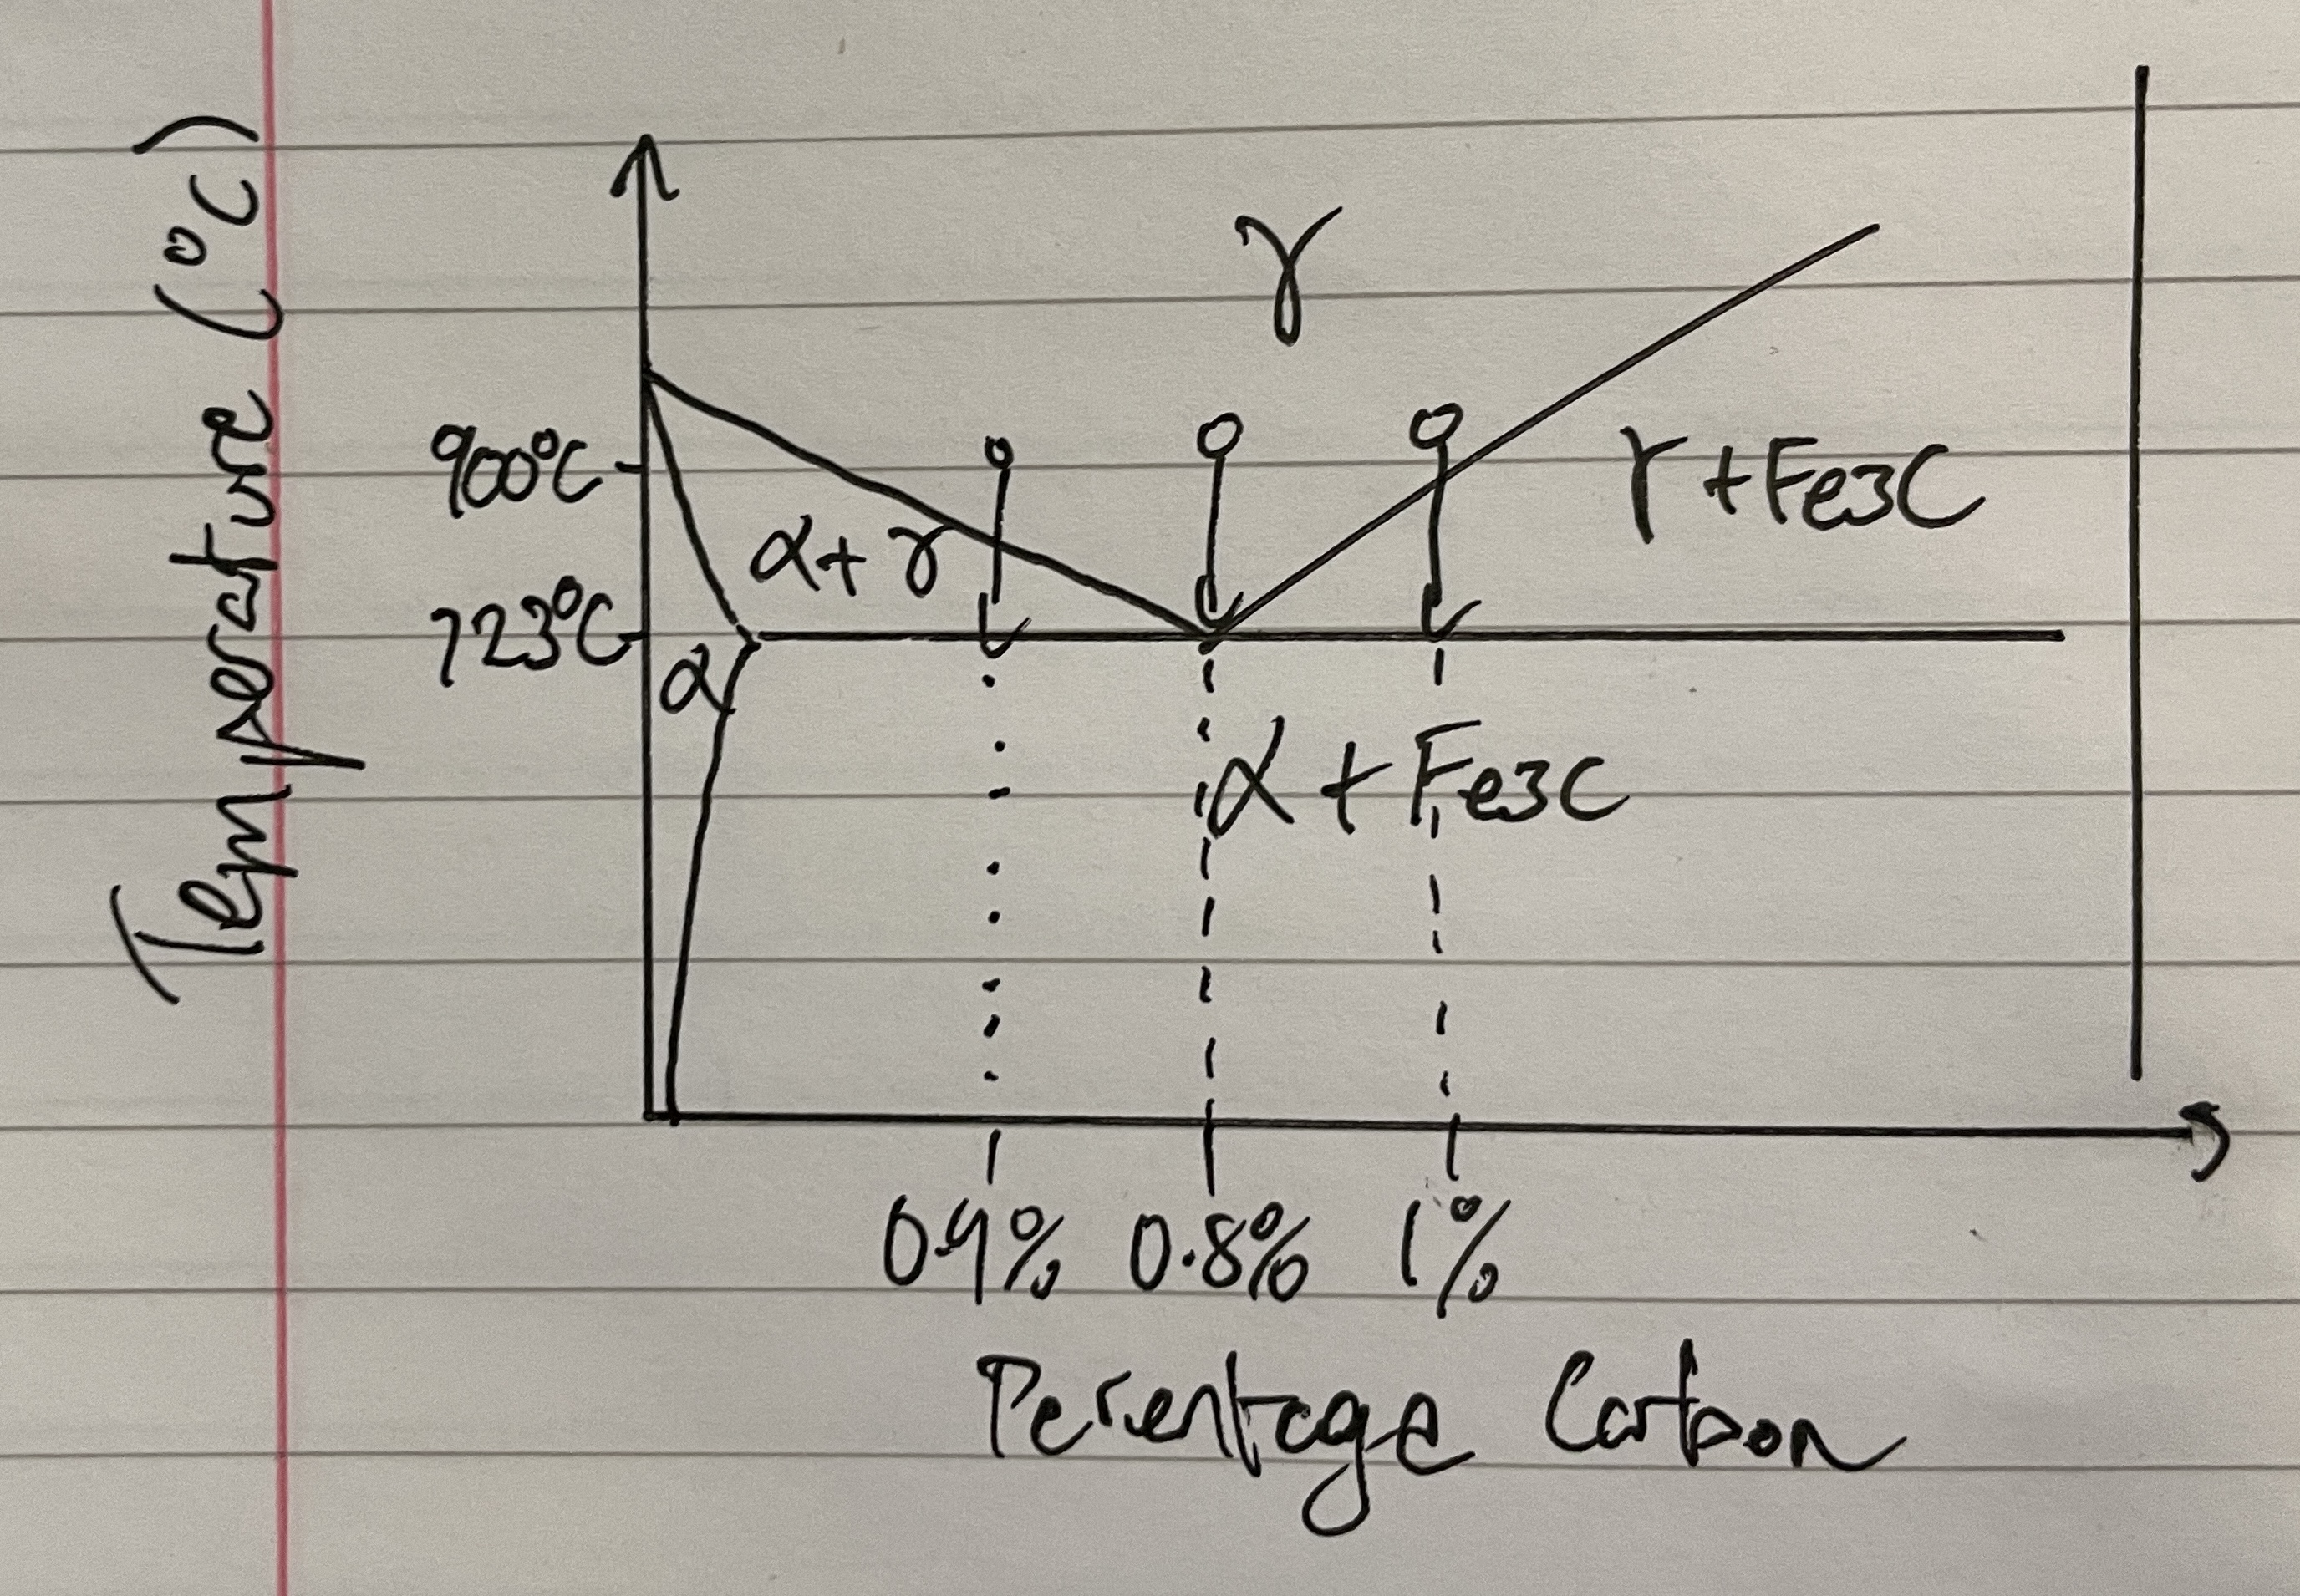
\includegraphics[width = 0.7\textwidth]{./img/q1b.jpg}
    \caption{Diagram showing cooling process.}
\end{figure}
\begin{figure}[H]
    \centering
    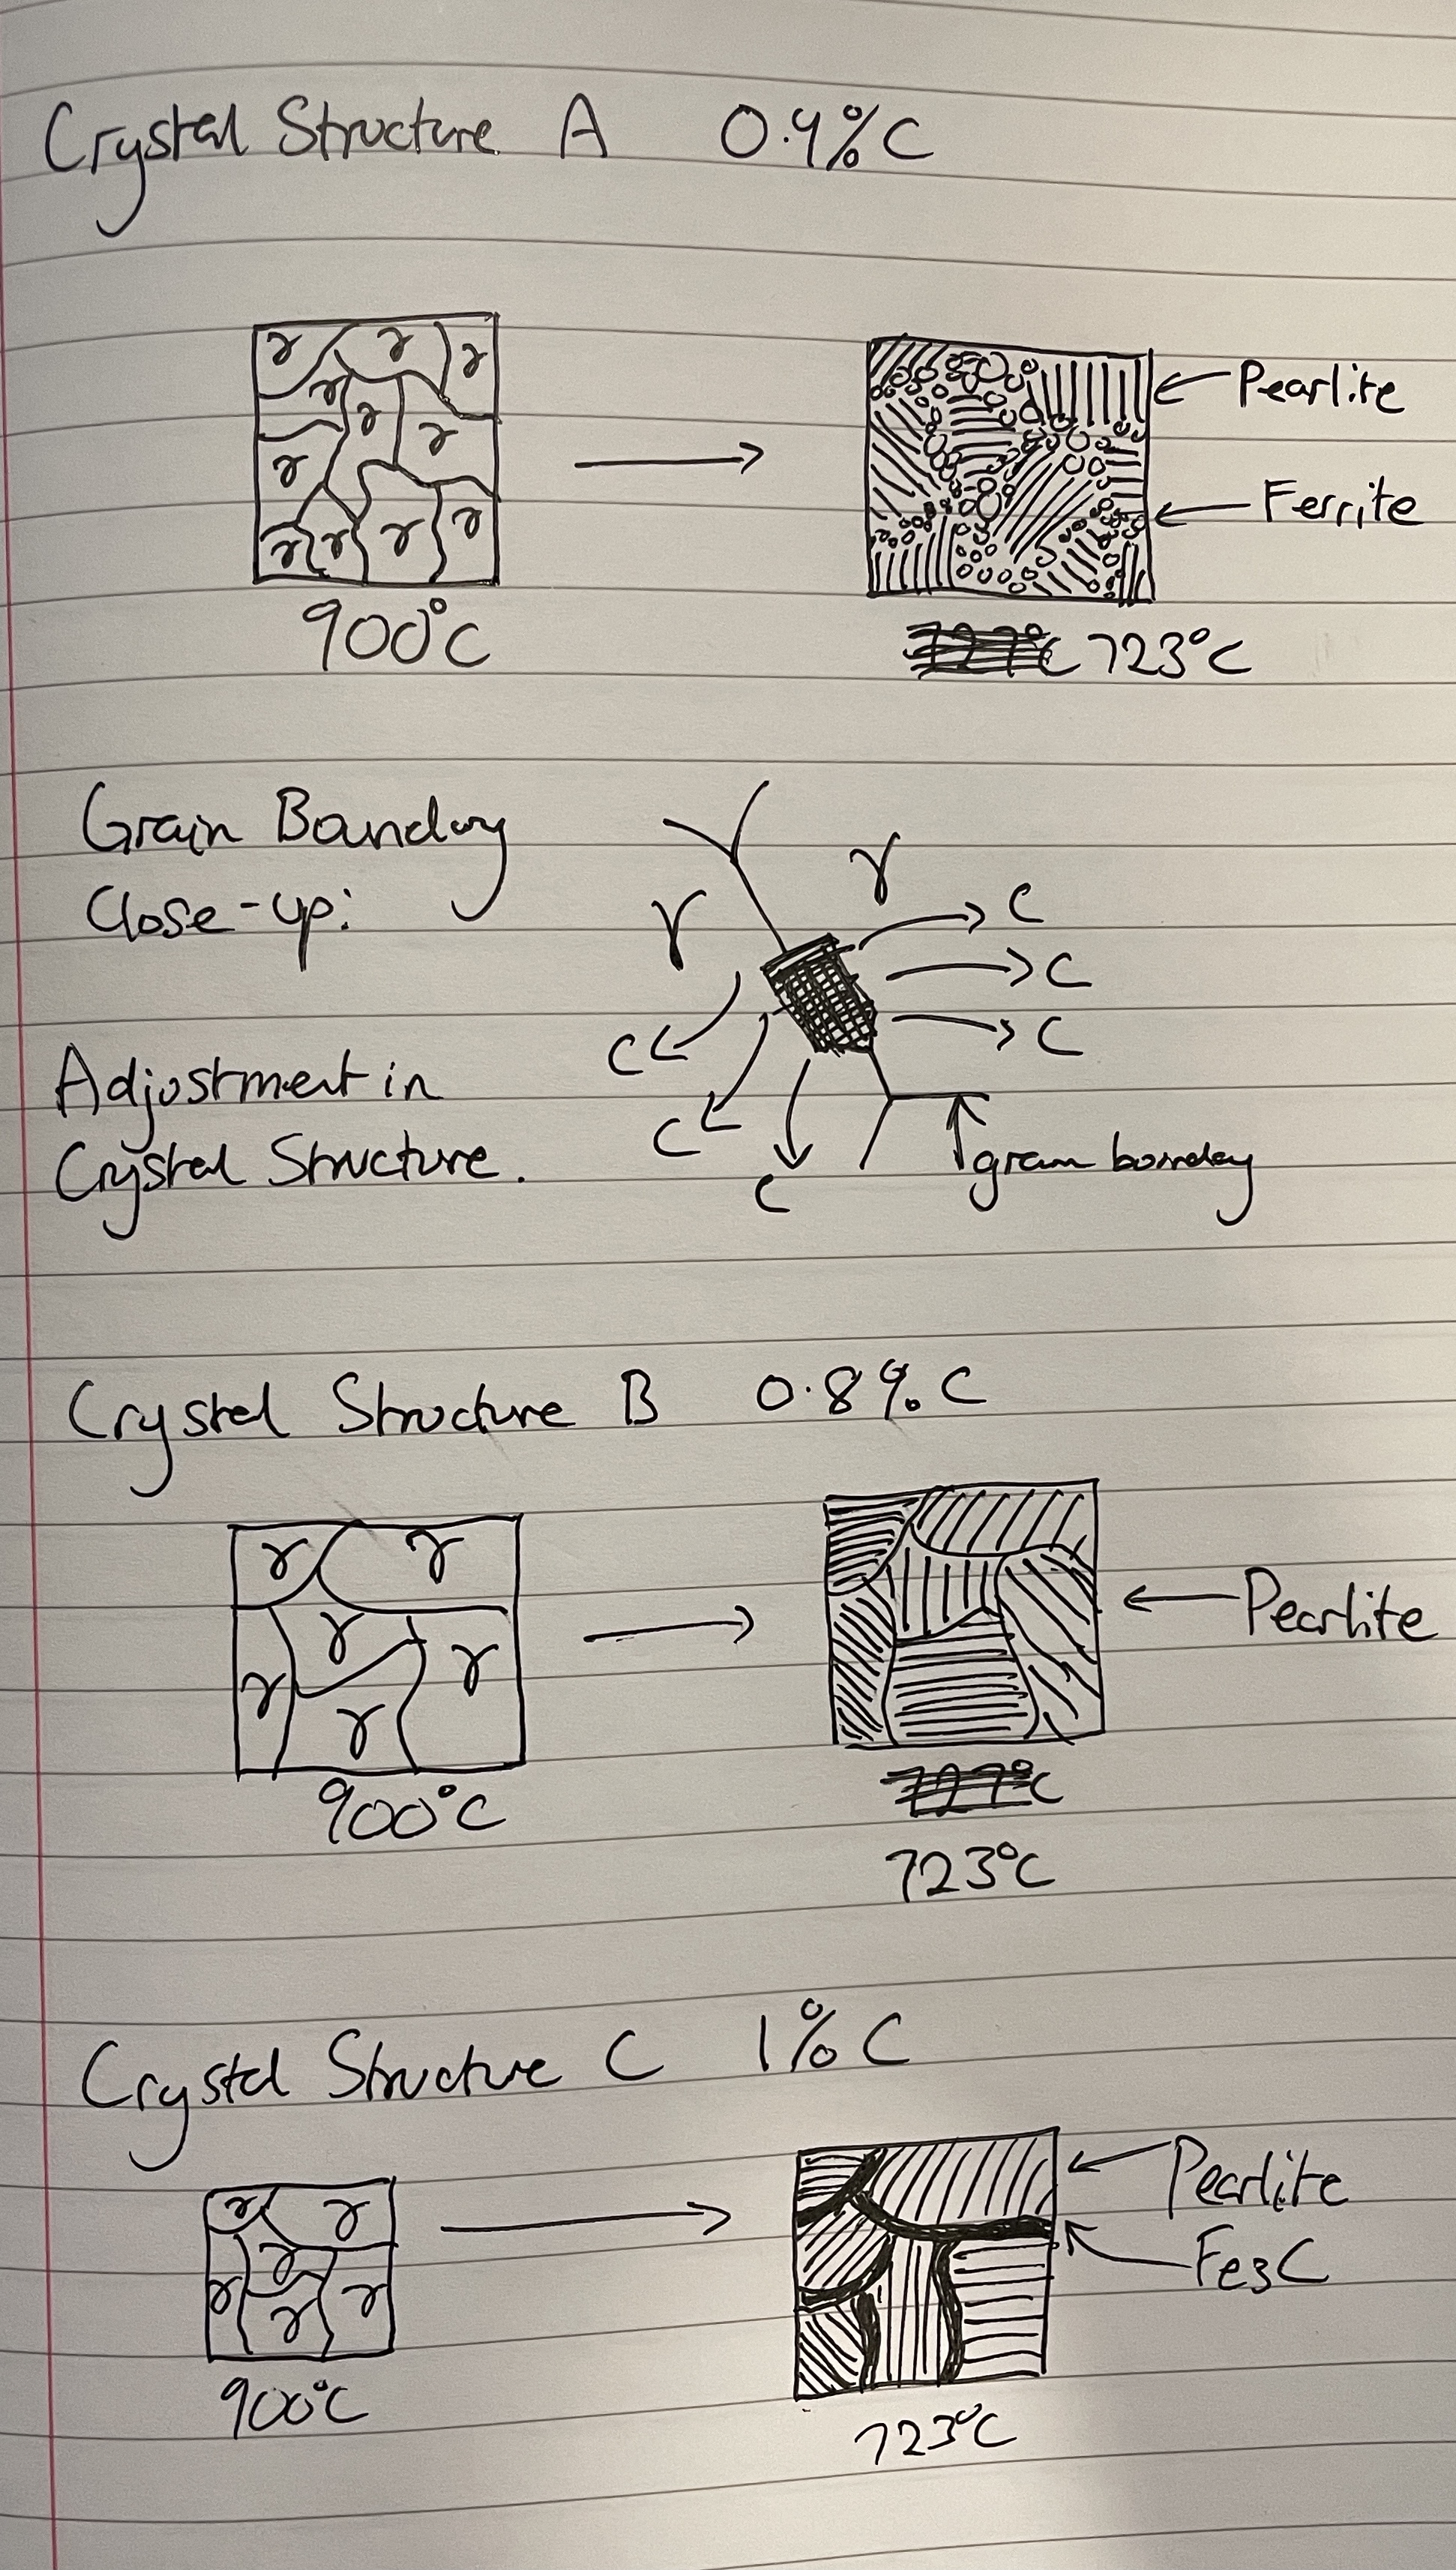
\includegraphics[height = 24cm]{./img/q1a.jpg}
    \caption{Diagrams showing how crystal structure changes with cooling from \SI{900}{\celsius} to \SI{723}{\celsius} for 0.4\%, 0.8\% and 1\% carbon content.}
\end{figure}

For 0.4\%, we can see the emergence of $\alpha$ forming at the grain boundary. This adjusts the crystal structure to form BCC areas and carbon must move away, enriching the $\gamma$ regions. This then converts the remaining $\gamma$ into pearlite as temperature decreases. With increasing carbon content, tensile strength increases as the pearlite is saturated (until 0.8\% carbon content is reached) as dislocations become more difficult in the microstructure. 

For 0.8\% carbon content, the crystal structure forms a 100\% pearlite crystal structure. This structure is tough as the pearlite is saturated with carbon and there is a fine grain boundary with no formation of $\alpha$ or \ce{Fe3C}.

For 1\% carbon content, we see a conversion of some of the $\gamma$ into \ce{Fe3C} at the grain boundary, leading to embrittlement. We know that $\gamma$ saturates at 0.8\% carbon content, so carbon moves away from $\gamma$ to form pearlite and \ce{Fe3C} at the grain boundaries (which has a higher carbon content), coating the pearlite crystals. This has the consequence that due to the positioning and location of the primary \ce{Fe3C}, the whole steel exhibits the toughness of \ce{Fe3C}. This toughness is lower than that of 100\% pearlite and hence is undesirable for tensile applications and should be avoided. 
\begin{figure}[H]
    \centering
    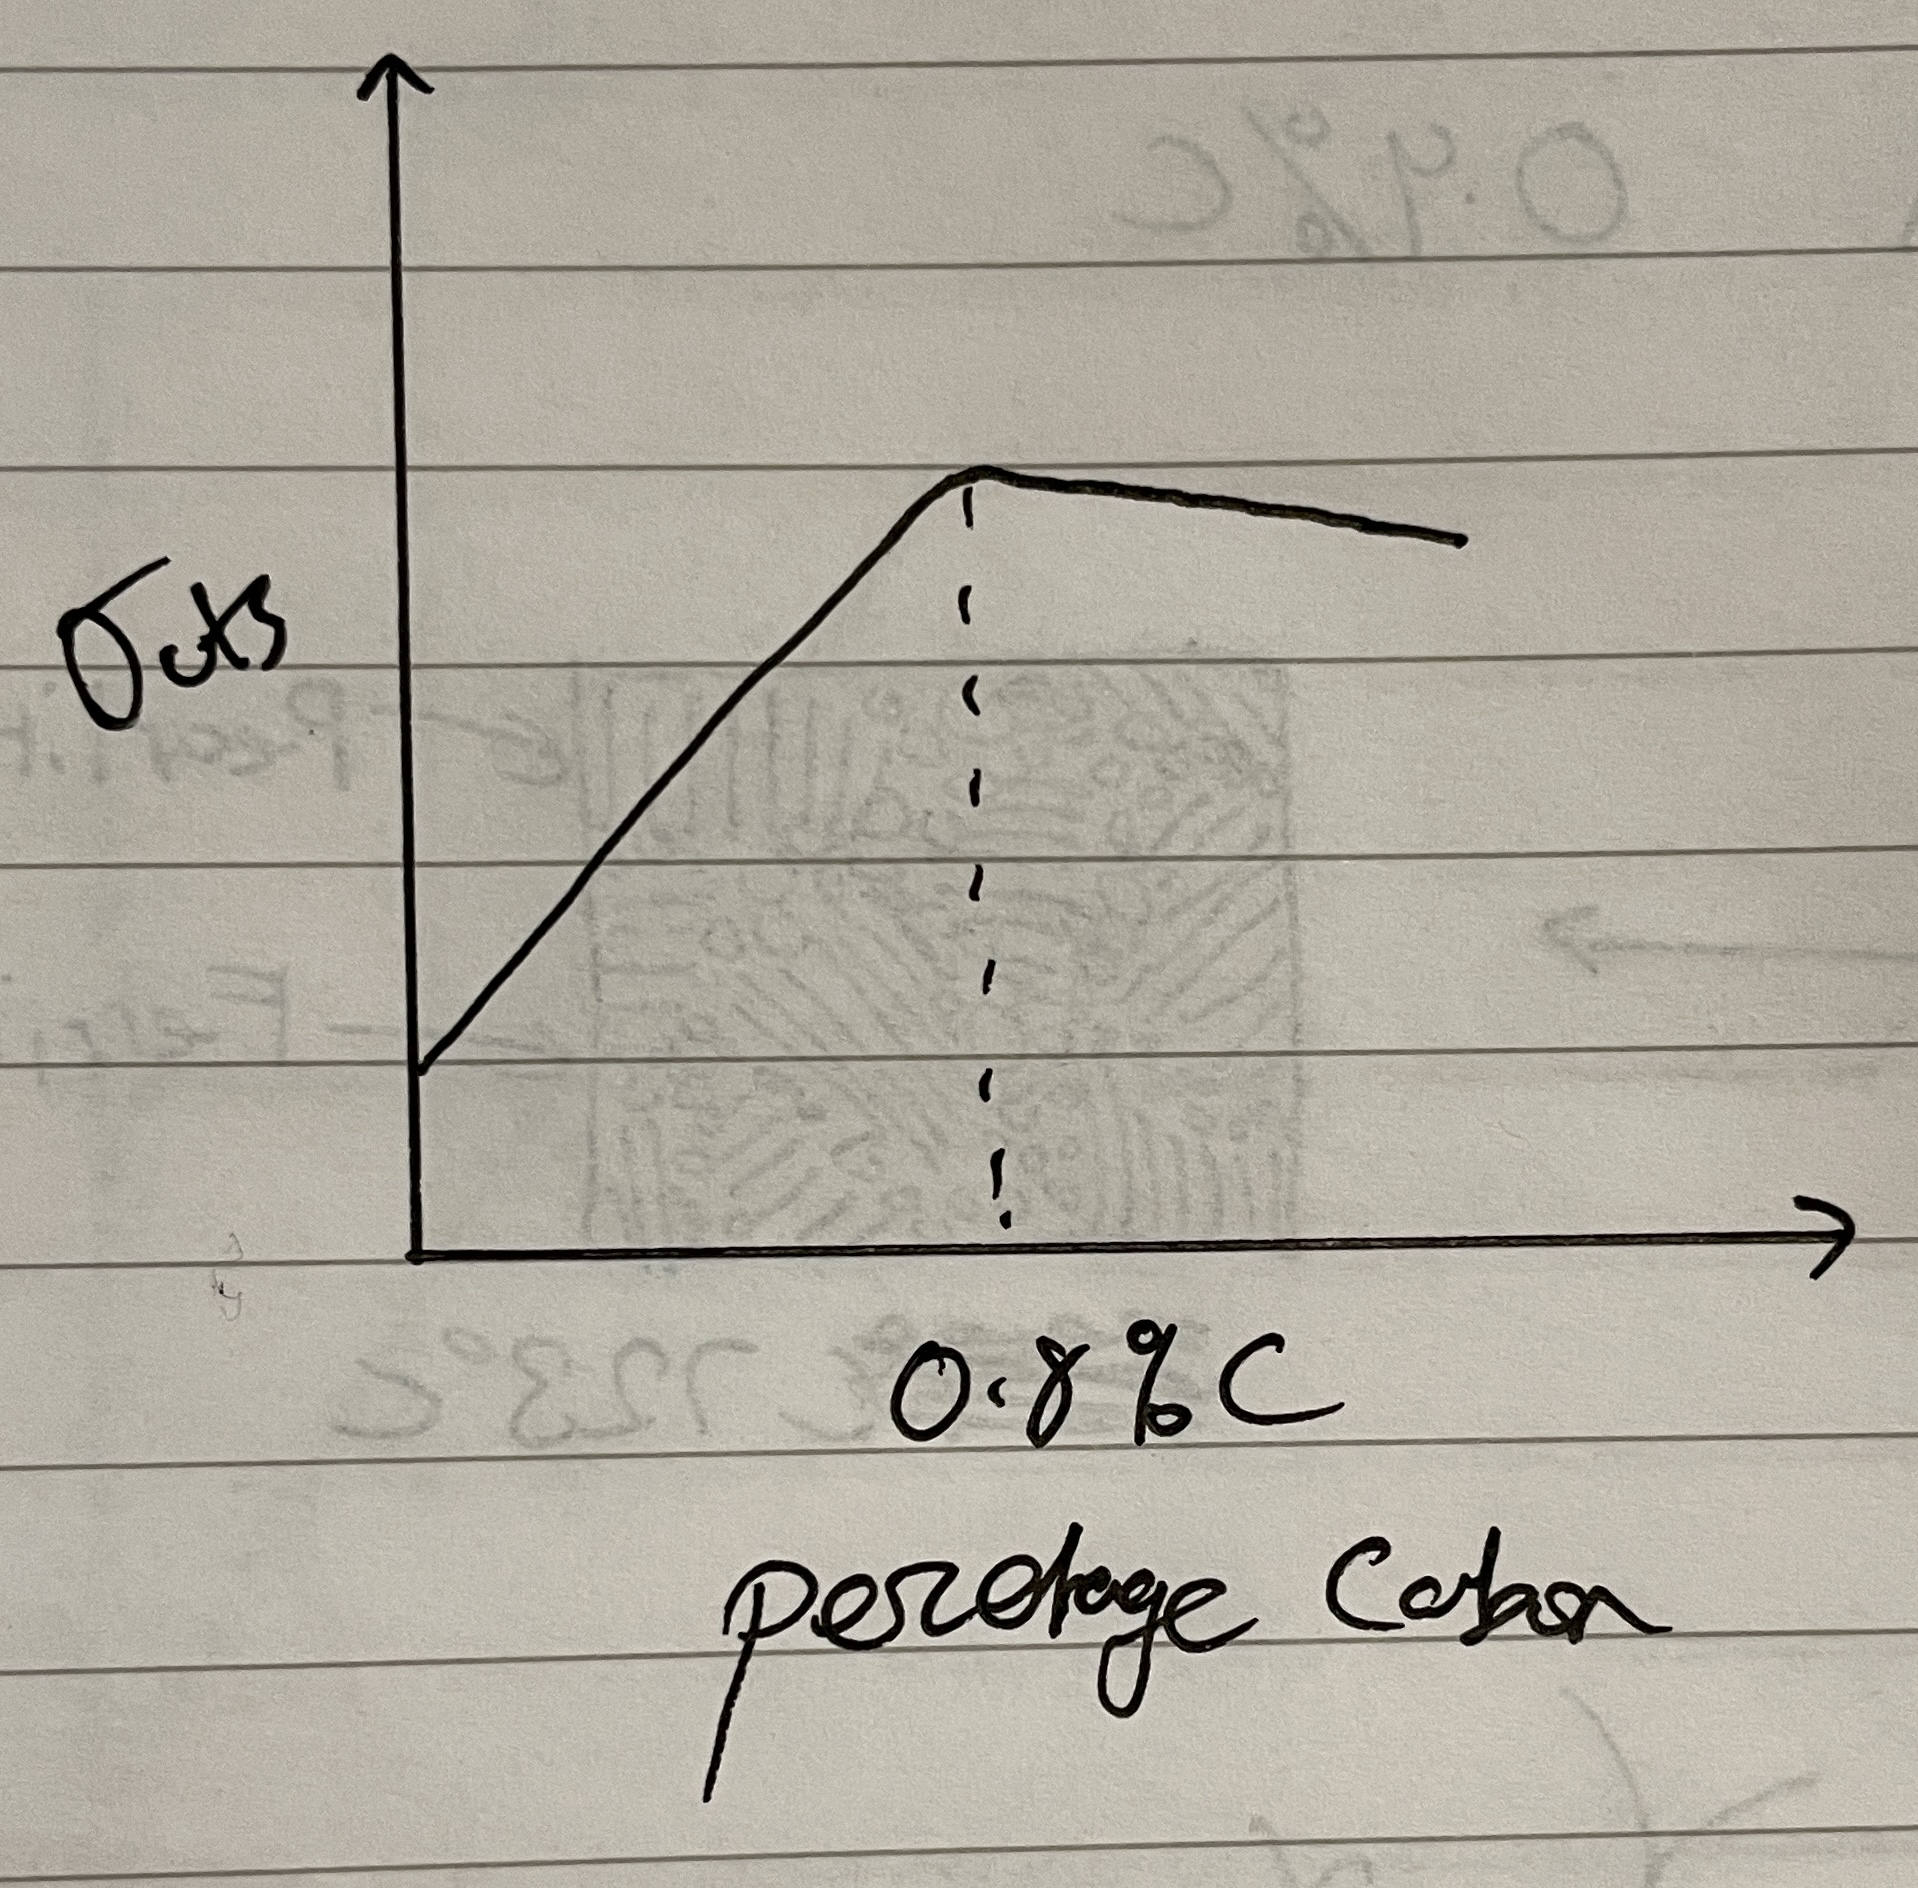
\includegraphics[width = 0.5\textwidth]{./img/q1c.jpg}
    \caption{Diagram showing how tensile strength varies with carbon content.}
\end{figure}
\section{Show that the area under the stress strain curve is equivalent to the elastic stored energy (in a stressed material). What part of the stress strain curve do you need?}
\section{Why is a process anneal (or stress relief anneal) not usually applied to steels above about 0.4\% carbon content? }
\section{Which way do we connect up the power supply in an impressed current cathodic protection scheme and why - and why should we still consider painting the buried pipelines as well (in addition to cathodically protecting it)?}
\end{document}